\documentclass{ximera}
\title{Graphics and interactives}
\author{Bart Snapp and Jason Nowell}
\begin{document}
\begin{abstract}
    How to include graphics and other interactive content.
\end{abstract}
\maketitle

\section{Including images}

In the last section, we showed you how to include images using \verb|includegraphics|. However, 
\textbf{The preferred method to include graphics is with TikZ.}
\begin{image}
  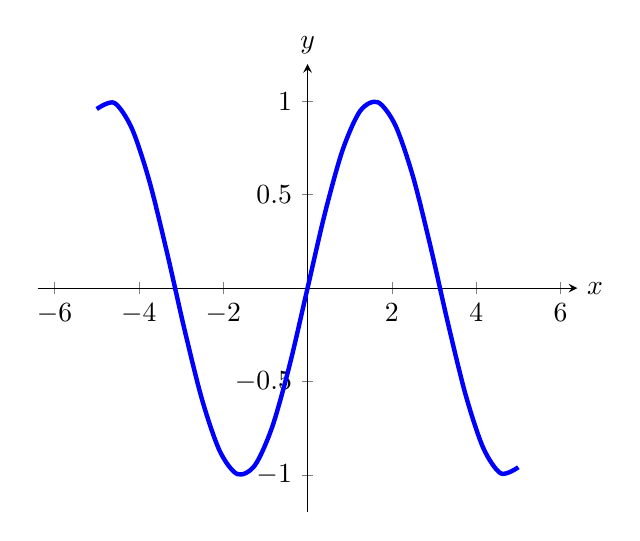
\begin{tikzpicture}
    \begin{axis}[
        xmin=-6.4,
        xmax=6.4,
        ymin=-1.2,
        ymax=1.2,
        axis lines=center,
        xlabel=$x$,
        ylabel=$y$,
        every axis y label/.style={at=(current axis.above origin),anchor=south},
        every axis x label/.style={at=(current axis.right of origin),anchor=west},
      ]
      \addplot [ultra thick, blue, smooth] {sin(deg(x))};
    \end{axis}
  \end{tikzpicture}
\end{image}
We can create the image above with the following code:
\begin{verbatim}
\begin{image}
  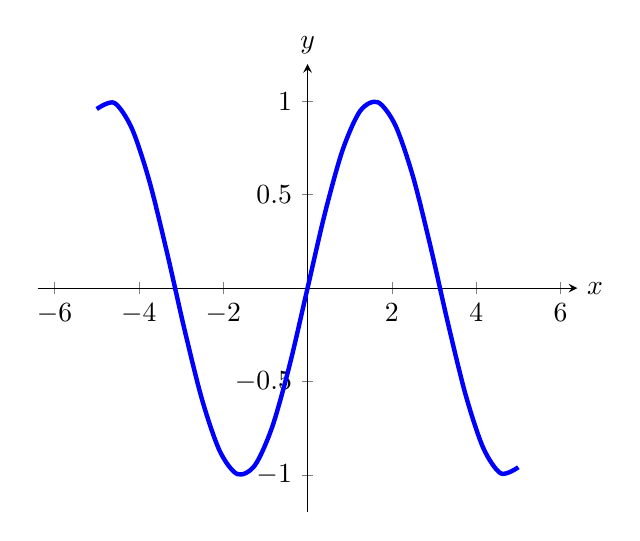
\begin{tikzpicture}
    \begin{axis}[
        xmin=-6.4,
        xmax=6.4,
        ymin=-1.2,
        ymax=1.2,
        axis lines=center,
        xlabel=$x$,
        ylabel=$y$,
        every axis y label/.style={at=(current axis.above origin),anchor=south},
        every axis x label/.style={at=(current axis.right of origin),anchor=west},
      ]
      \addplot [ultra thick, blue, smooth] {sin(deg(x))};
    \end{axis}
  \end{tikzpicture}
\end{image}
\end{verbatim}



\section{Videos}

We can embed YouTube Videos with 

\verb|\youtube{FvgF95i0_lw}| which would embed the video into the page, like this:
\begin{center}
        \youtube{FvgF95i0_lw}
\end{center}



\section{The graph command}

The easiest way to include an interactive graph is to use the
\verb|\graph| command. Unfortunately, the \verb|\graph| command
doesn't draw a graph in the PDF, rather, it states (in words) that a
graph is produced.
\[
\graph{x^2}
\]
There are a number of options for the \verb|\graph| command, and you can find out more WHERE?
Here are two examples. One with axis labels and a set window:  

\[
\graph[xAxisLabel="time", yAxisLabel="distance",xmin=0, xmax=10, ymin=0, ymax=10]{y=x^3}
\]
coded via:
\begin{verbatim}
\[
\graph[xAxisLabel="time", yAxisLabel="distance",xmin=0, xmax=2, ymin=0, ymax=10]{y=x^3}
\]
\end{verbatim}

and another, piecewise function:
\[
\graph{ \sin(x)\left\{x<0\right\}, 2x\left\{ x>=0 \right\} }
\]
coded via:
\begin{verbatim}
\[
\graph{ \sin(x)\left\{x<0\right\}, 2x\left\{ x>=0 \right\} }
\]
\end{verbatim}


\section{Desmos}

If you require further features from
\link[Desmos]{https://www.desmos.com/}, you can sign up for an account
and include your worksheets like this:

\begin{verbatim}
\begin{center}
\desmos{zwywds7med}{800}{600}
\end{center}
\end{verbatim}
\begin{center}
\desmos{zwywds7med}{800}{600}
\end{center}


  \section{How to embed GeoGebra}

        You can also use \link[GeoGebra]{https://www.geogebra.org/}. Embed the
        widget using the syntax \verb|\geogebra{ID}{width}{height}|, where ID
        is the widget ID and width and height are the dimensions (in pixels)
        you want the embedded widget to have.
        
    
        \begin{center}
            \geogebra{XC3FXUdJ}{800}{600}%%https://www.geogebra.org/m/XC3FXUdJ
        \end{center}
        
        The above embedding is generated via the code:
        
        \begin{verbatim}
            \begin{center}
            \geogebra{XC3FXUdJ}{800}{600}
            \end{center}
        \end{verbatim}      

        \section{How to embed Desmos 3D}

        \begin{center}
          \desmosThreeD{bb4exrhrl3}{800}{600}
        \end{center}
        \begin{verbatim}
          \begin{center}
          \desmosThreeD{bb4exrhrl3}{800}{600}
          \end{center}
      \end{verbatim}    
      






\end{document}
